\chapter{Hardware Calculations}
\section{Fuse Calculations}
%I am adding a table here for calculations
%finally...
%i am
\begin{center}
	%   \setlength\extrarowheight{7pt}
	\begin{tabular}{c|c|c}
		\toprule
		{\large Element} & {Quantity} & {\large Maximum Power Consumption (Watt)} \\\midrule
		%\vspace{0.7mm}
		{\large Raspberry Pi 4} & {\large 1} & {\large 6.4}\\
		{\large DC Motor} & {4} & {\large 25.2} \\
		{\large Servo Motor MG996R} & {\large 2} & {\large 15} \\
		{\large USB Camera} & {\large 1} & {\large 1.25} \\
		{\large Miscellaneous} &{\large ---} & {\large 2} \\ 
		\bottomrule
	\end{tabular}
\end{center}
For a maximum input voltage = \textbf{12.6 V}, and a maximum efficiency of the buck = \textbf{95\%}.

$\because$ The only loads supplied directly from the battery pack are the DC motors, while the rest is powered form the \textbf{5 V} buck converter.

$\therefore$ Current draw from the converter is:
\begin{equation}
	I_{5 V} = \frac{6.4 + 15 + 1.25 + 2}{5} = 4.93 A  
\end{equation}

Multiplying by a safety factor of \textbf{1.25}, we get a fuse rating of \textbf{6.1625 A}. $\therefore$ A \textbf{6 A} fuse is placed after the converter.

Similarly, the total current drawn from the pack is:
\begin{equation}
	I_{total} = \frac{6.4 + 15 + 1.25 + 2}{12.6 * 0.95} + \frac{25.2}{12.6} = 4.06 A  
\end{equation}
Multiplying by a safety factor of \textbf{1.25}, we get a fuse rating of \textbf{5.074 A}. $\therefore$ A \textbf{5 A} fuse is placed after the BMS.






\section{Voltage Measurement}
As explained in section \ref{sec:bat-man}, voltage measurement depends on measuring the middle voltages of voltage divider, powered by different sections of the the pack as shown in figure \ref{fig:hw-volt-mes-apenC}

\begin{figure}[h!]
	\centering
	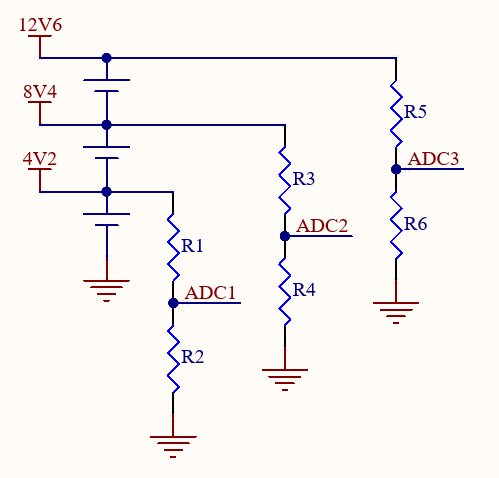
\includegraphics[scale=0.5]{./Figures/HW/Voltage-Measurement.png}
	\caption{Voltage Measurement Using Voltage Divider}
	\label{fig:hw-volt-mes-apenC}
\end{figure}

To determine suitable values for the resistors, some givens are determined:
\begin{itemize}
	\item Each module is charged to its full capacity (i.e. the voltage of each module = \textbf{4.2 V}).
	\item The middle voltage corresponding to the maximum input voltage = \textbf{3.3 V}.
\end{itemize}
Starting with the nearest module to ground, the relation between \textbf{4V2} and \textbf{ADC1} is:
\begin{equation}
	ADC1 = 4V2*\frac{R_2}{R_1 + R_2}
\end{equation}
Substituting by numbers and rearranging:
\begin{equation}
	\frac{R_2}{R_1 + R_2} = \frac{11}{14} 
\end{equation}

\begin{equation}
	11*R_1 + 11*R_2 = 14*R_2
\end{equation}

To achieve the desired output, the relation between \textbf{$R_1$} and \textbf{$R_2$} is:
\begin{equation}
	\frac{R_1}{R_2} = \frac{3}{11} \approxeq 0.27273
\end{equation}
Similarly, the relations related to the second  and third voltage divider are : 

\begin{equation}
	ADC2 = 8V4*\frac{R_4}{R_3 + R_4}
\end{equation}

\begin{equation}
	ADC3 = 12V6*\frac{R_6}{R_5 + R_6}
\end{equation}

Following with the same logic as in the first voltage divider, the resulting relations are:
\begin{equation}
	\frac{R_3}{R_4} = \frac{17}{11} \approxeq 1.5454
\end{equation}

\begin{equation}
	\frac{R_5}{R_6} = \frac{31}{11} \approxeq 2.8181
\end{equation}
It is worth mentioning that these ratios are hard to achieve practically, as well as it can be risky to use resistors that result in a slightly lower ratios, risking the controller. It is easier and safer to use higher ratios to decrease the maximum value of \textbf{ADCn}, but not so high to utilize a large range of the ADC.
\newline As a result, the values of resistors from \textbf{$R_1$} to \textbf{$R_6$} are: \{10, 22, 56, 33, 33, 10\} $k\Omega$, to achieve the ratios of approximately: {0.45454, 1.69697, 3.3} respectively.

\section{Current Measurement}
For current measurement using a shunt resistor, a very low voltage drop is desired. Assuming a voltage drop across $R_{shunt}$ = \textbf{0.1 V}, a shunt of $25 m\Omega$ is used. However, a $100 m\Omega$ is available locally. Therefore two of these in parallel are connected for about a $50 m\Omega$ shunt, with \textbf{0.2 V}.

To increase the voltage range for the ADC, a non-inverting amplifier is used. For a maximum output voltage of \textbf{3 V}, the gain of the op-amp can be:
\begin{equation}
	G = \frac{3 V}{0.2 V} = 15 V/V
\end{equation}
$\because$ The relation of a non-inverting amplifier is:
\begin{equation}
	G = 1 + \frac{R_f}{R_1}
\end{equation}
$\therefore$ a ratio $\frac{R_f}{R_1}$ of 14 is needed. Values of $R_f$ and $R_1$ can be \textbf{$150k\Omega$} and \textbf{$15k\Omega$} respectively.

\section{Temperature Measurement}

\begin{figure}[h!]
	\centering
	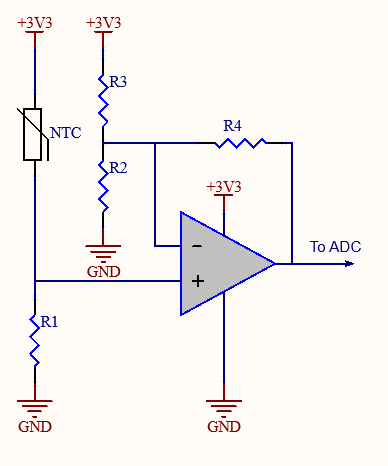
\includegraphics[scale=0.5]{./Figures/HW/Temperature Measurement.png}
	\caption{Temperature Measurement Using Op-Amp \cite{op_amp_temperature}}
	\label{fig:hw-temp-mes-append}
\end{figure}

Based on the document provided by \textbf{Texas Instruments} \cite{op_amp_temperature}, The following givens are stated:
\begin{itemize}
	\item $T_{min} = 20 $\textdegree C , $T_{max} = 42\textdegree$ \textdegree C.
	\item $Vout_{min} = 0.5 V$, $Vout_{max} = 3.25 V$.
	\item $V_{dd} = 3.3 V$
\end{itemize}
$\therefore$ $NTC_{max} = 125 k\Omega$, $NTC_{min} = 50 k\Omega$.
$\therefore R_1 \approxeq 78 k\Omega$.
Calculating $Vin_{max}$, and $Vin_{min}$:
\begin{equation}
	Vin_{min} = V_{dd} * \frac{R_1}{NTC_{max} + R_1} = 1.267 V
\end{equation}
\begin{equation}
	Vin_{max} = V_{dd} * \frac{R_1}{NTC_{min} + R_1} = 2.01 V
\end{equation}
Calculating the Ideal Gain:
\begin{equation}
	G_{ideal} = \frac{Vout_{max} - Vout_{min}}{Vin_{max} - Vin_{min}} = 3.701 V/V
\end{equation}
Assuming a value for $R_4 = 68 k\Omega$, solving for $R_2$ and $R_3$:
\begin{equation}
	R_2 || R_3 = \frac{R_4}{G_{ideal} - 1} \approxeq 25176 k\Omega
\end{equation}

\begin{equation}
	R_3 = \frac{ R_4 * V_{dd} }{ Vin_{max}*G_{ideal} - Vout_{max} } = 
\end{equation}

\begin{equation}
	R_3 = \frac{ (R_2 || R_3)_{ideal}*R_3 }{ R_3 - (R_2 || R_3)_{ideal} } \approxeq 53568 k\Omega. The closest standard value = 56 k\Omega
\end{equation}


\begin{equation}
	R_2 = \frac{ (R_2 || R_3)_{ideal}*R_3 }{ R_3 - (R_2 || R_3)_{ideal} } \approxeq 47499 k\Omega. The closest standard value = 47 k\Omega
\end{equation}

